% Options for packages loaded elsewhere
\PassOptionsToPackage{unicode}{hyperref}
\PassOptionsToPackage{hyphens}{url}
\documentclass[
]{article}
\usepackage{xcolor}
\usepackage[margin=1in]{geometry}
\usepackage{amsmath,amssymb}
\setcounter{secnumdepth}{-\maxdimen} % remove section numbering
\usepackage{iftex}
\ifPDFTeX
  \usepackage[T1]{fontenc}
  \usepackage[utf8]{inputenc}
  \usepackage{textcomp} % provide euro and other symbols
\else % if luatex or xetex
  \usepackage{unicode-math} % this also loads fontspec
  \defaultfontfeatures{Scale=MatchLowercase}
  \defaultfontfeatures[\rmfamily]{Ligatures=TeX,Scale=1}
\fi
\usepackage{lmodern}
\ifPDFTeX\else
  % xetex/luatex font selection
\fi
% Use upquote if available, for straight quotes in verbatim environments
\IfFileExists{upquote.sty}{\usepackage{upquote}}{}
\IfFileExists{microtype.sty}{% use microtype if available
  \usepackage[]{microtype}
  \UseMicrotypeSet[protrusion]{basicmath} % disable protrusion for tt fonts
}{}
\makeatletter
\@ifundefined{KOMAClassName}{% if non-KOMA class
  \IfFileExists{parskip.sty}{%
    \usepackage{parskip}
  }{% else
    \setlength{\parindent}{0pt}
    \setlength{\parskip}{6pt plus 2pt minus 1pt}}
}{% if KOMA class
  \KOMAoptions{parskip=half}}
\makeatother
\usepackage{color}
\usepackage{fancyvrb}
\newcommand{\VerbBar}{|}
\newcommand{\VERB}{\Verb[commandchars=\\\{\}]}
\DefineVerbatimEnvironment{Highlighting}{Verbatim}{commandchars=\\\{\}}
% Add ',fontsize=\small' for more characters per line
\usepackage{framed}
\definecolor{shadecolor}{RGB}{248,248,248}
\newenvironment{Shaded}{\begin{snugshade}}{\end{snugshade}}
\newcommand{\AlertTok}[1]{\textcolor[rgb]{0.94,0.16,0.16}{#1}}
\newcommand{\AnnotationTok}[1]{\textcolor[rgb]{0.56,0.35,0.01}{\textbf{\textit{#1}}}}
\newcommand{\AttributeTok}[1]{\textcolor[rgb]{0.13,0.29,0.53}{#1}}
\newcommand{\BaseNTok}[1]{\textcolor[rgb]{0.00,0.00,0.81}{#1}}
\newcommand{\BuiltInTok}[1]{#1}
\newcommand{\CharTok}[1]{\textcolor[rgb]{0.31,0.60,0.02}{#1}}
\newcommand{\CommentTok}[1]{\textcolor[rgb]{0.56,0.35,0.01}{\textit{#1}}}
\newcommand{\CommentVarTok}[1]{\textcolor[rgb]{0.56,0.35,0.01}{\textbf{\textit{#1}}}}
\newcommand{\ConstantTok}[1]{\textcolor[rgb]{0.56,0.35,0.01}{#1}}
\newcommand{\ControlFlowTok}[1]{\textcolor[rgb]{0.13,0.29,0.53}{\textbf{#1}}}
\newcommand{\DataTypeTok}[1]{\textcolor[rgb]{0.13,0.29,0.53}{#1}}
\newcommand{\DecValTok}[1]{\textcolor[rgb]{0.00,0.00,0.81}{#1}}
\newcommand{\DocumentationTok}[1]{\textcolor[rgb]{0.56,0.35,0.01}{\textbf{\textit{#1}}}}
\newcommand{\ErrorTok}[1]{\textcolor[rgb]{0.64,0.00,0.00}{\textbf{#1}}}
\newcommand{\ExtensionTok}[1]{#1}
\newcommand{\FloatTok}[1]{\textcolor[rgb]{0.00,0.00,0.81}{#1}}
\newcommand{\FunctionTok}[1]{\textcolor[rgb]{0.13,0.29,0.53}{\textbf{#1}}}
\newcommand{\ImportTok}[1]{#1}
\newcommand{\InformationTok}[1]{\textcolor[rgb]{0.56,0.35,0.01}{\textbf{\textit{#1}}}}
\newcommand{\KeywordTok}[1]{\textcolor[rgb]{0.13,0.29,0.53}{\textbf{#1}}}
\newcommand{\NormalTok}[1]{#1}
\newcommand{\OperatorTok}[1]{\textcolor[rgb]{0.81,0.36,0.00}{\textbf{#1}}}
\newcommand{\OtherTok}[1]{\textcolor[rgb]{0.56,0.35,0.01}{#1}}
\newcommand{\PreprocessorTok}[1]{\textcolor[rgb]{0.56,0.35,0.01}{\textit{#1}}}
\newcommand{\RegionMarkerTok}[1]{#1}
\newcommand{\SpecialCharTok}[1]{\textcolor[rgb]{0.81,0.36,0.00}{\textbf{#1}}}
\newcommand{\SpecialStringTok}[1]{\textcolor[rgb]{0.31,0.60,0.02}{#1}}
\newcommand{\StringTok}[1]{\textcolor[rgb]{0.31,0.60,0.02}{#1}}
\newcommand{\VariableTok}[1]{\textcolor[rgb]{0.00,0.00,0.00}{#1}}
\newcommand{\VerbatimStringTok}[1]{\textcolor[rgb]{0.31,0.60,0.02}{#1}}
\newcommand{\WarningTok}[1]{\textcolor[rgb]{0.56,0.35,0.01}{\textbf{\textit{#1}}}}
\usepackage{longtable,booktabs,array}
\usepackage{calc} % for calculating minipage widths
% Correct order of tables after \paragraph or \subparagraph
\usepackage{etoolbox}
\makeatletter
\patchcmd\longtable{\par}{\if@noskipsec\mbox{}\fi\par}{}{}
\makeatother
% Allow footnotes in longtable head/foot
\IfFileExists{footnotehyper.sty}{\usepackage{footnotehyper}}{\usepackage{footnote}}
\makesavenoteenv{longtable}
\usepackage{graphicx}
\makeatletter
\newsavebox\pandoc@box
\newcommand*\pandocbounded[1]{% scales image to fit in text height/width
  \sbox\pandoc@box{#1}%
  \Gscale@div\@tempa{\textheight}{\dimexpr\ht\pandoc@box+\dp\pandoc@box\relax}%
  \Gscale@div\@tempb{\linewidth}{\wd\pandoc@box}%
  \ifdim\@tempb\p@<\@tempa\p@\let\@tempa\@tempb\fi% select the smaller of both
  \ifdim\@tempa\p@<\p@\scalebox{\@tempa}{\usebox\pandoc@box}%
  \else\usebox{\pandoc@box}%
  \fi%
}
% Set default figure placement to htbp
\def\fps@figure{htbp}
\makeatother
\setlength{\emergencystretch}{3em} % prevent overfull lines
\providecommand{\tightlist}{%
  \setlength{\itemsep}{0pt}\setlength{\parskip}{0pt}}
\usepackage{bookmark}
\IfFileExists{xurl.sty}{\usepackage{xurl}}{} % add URL line breaks if available
\urlstyle{same}
\hypersetup{
  pdftitle={Spatial Analysis of breast cancer tumor microenvironment},
  pdfauthor={Aymen Maqsood},
  hidelinks,
  pdfcreator={LaTeX via pandoc}}

\title{Spatial Analysis of breast cancer tumor microenvironment}
\author{Aymen Maqsood}
\date{2025-01-23}

\begin{document}
\maketitle

\begin{Shaded}
\begin{Highlighting}[]
\NormalTok{knitr}\SpecialCharTok{::}\NormalTok{opts\_chunk}\SpecialCharTok{$}\FunctionTok{set}\NormalTok{(}
\AttributeTok{warning =} \ConstantTok{FALSE}\NormalTok{,}
\AttributeTok{message =} \ConstantTok{FALSE}\NormalTok{,}
\AttributeTok{echo =} \ConstantTok{TRUE}  \CommentTok{\# Show code in the output}
\NormalTok{)}
\end{Highlighting}
\end{Shaded}

\section{Spatial Data Analysis Report: Xenium Human Breast Cancer
Dataset}\label{spatial-data-analysis-report-xenium-human-breast-cancer-dataset}

Independent Project of analysis workflow performed to study the spatial
transcriptomics of a human breast cancer dataset generated using the
Xenium platform. The analysis follows standard steps like:

\begin{itemize}
\tightlist
\item
  \textbf{Data Preprocessing}
\item
  \textbf{Normalization}
\item
  \textbf{Dimensionality Reduction}
\item
  \textbf{Clustering}
\item
  \textbf{Cell Type Annotation}
\item
  \textbf{Spatial Visualization}
\end{itemize}

\subsection{Key Findings}\label{key-findings}

The analysis found distinct cell populations, with invasive carcinoma
cells concentrated in specific areas, potentially indicating tumor
boundaries. FAS expression was notably high in these invasive regions,
surprising given its role in tumor metabolism, while CEACAM6 marked
ductal carcinoma areas. Immune cells were scattered, suggesting
infiltration into the tumor.

\subsection{Introduction}\label{introduction}

The Xenium platform is a spatial transcriptomics technology that allows
for the simultaneous measurement of gene expression and spatial location
of cells in a tissue section. The dataset contains gene expression data
from thousands of cells, as well as spatial information about the
location of each cell in the tissue section. In this analysis, we will
conduct a comprehensive analysis of the Dataset to identify cell types,
spatial patterns, and marker genes associated with breast cancer.

\textbf{Data Source:}:
\url{https://www.10xgenomics.com/products/xenium-in-situ/preview-dataset-human-breast}

\subsubsection{Loading Packages}\label{loading-packages}

\begin{Shaded}
\begin{Highlighting}[]
\FunctionTok{library}\NormalTok{(Seurat)}
\FunctionTok{library}\NormalTok{(tidyverse)}
\FunctionTok{library}\NormalTok{(SeuratObject)}
\end{Highlighting}
\end{Shaded}

\subsubsection{Loading Data}\label{loading-data}

\begin{Shaded}
\begin{Highlighting}[]
\NormalTok{xenium.obj }\OtherTok{\textless{}{-}} \FunctionTok{LoadXenium}\NormalTok{(}
  \StringTok{"\textasciitilde{}/Desktop/Projects/V1.0/Spatial{-}scRNA{-}Seq/Xenium Human Breast Cancer Dataset/data/outs/"}\NormalTok{,}
  \AttributeTok{fov =} \StringTok{"fov"}\NormalTok{, }
  \AttributeTok{assay =} \StringTok{"Xenium"}
\NormalTok{)}
\end{Highlighting}
\end{Shaded}

\subsubsection{Data Preprocessing / Quality
Control}\label{data-preprocessing-quality-control}

Initial preprocessing removes low-quality cells and visualizes key
metrics:

\begin{itemize}
\tightlist
\item
  \textbf{Remove cells with zero counts:} Ensures only cells with
  detectable transcripts are analyzed.
\item
  \textbf{Visualize distributions:} Violin plots display genes per cell
  (\texttt{nFeature\_Xenium}) and transcript counts per cell
  (\texttt{nCount\_Xenium}).
\item
  \textbf{Filtering:} Cells are subsetted to retain those with 5--200
  features and 10--1000 counts, reducing noise from low-quality cells or
  outliers.
\end{itemize}

\begin{Shaded}
\begin{Highlighting}[]
\CommentTok{\# remove cells with 0 counts}
\NormalTok{xenium.obj }\OtherTok{\textless{}{-}} \FunctionTok{subset}\NormalTok{(xenium.obj, }\AttributeTok{subset =}\NormalTok{ nCount\_Xenium }\SpecialCharTok{\textgreater{}} \DecValTok{0}\NormalTok{)}

\CommentTok{\# Genes/cell (nFeature\_Xenium) and transcript counts/cell (nCount\_Xenium)}
\FunctionTok{VlnPlot}\NormalTok{(xenium.obj, }\AttributeTok{features =} \FunctionTok{c}\NormalTok{(}\StringTok{"nFeature\_Xenium"}\NormalTok{, }\StringTok{"nCount\_Xenium"}\NormalTok{), }
        \AttributeTok{ncol =} \DecValTok{2}\NormalTok{, }\AttributeTok{pt.size =} \DecValTok{0}\NormalTok{)}
\end{Highlighting}
\end{Shaded}

\pandocbounded{\includegraphics[keepaspectratio]{Sample_report_DFCI_files/figure-latex/unnamed-chunk-4-1.pdf}}

\begin{Shaded}
\begin{Highlighting}[]
\CommentTok{\# Save the plot}
\FunctionTok{ggsave}\NormalTok{(}\StringTok{"VlnPlot\_QC.png"}\NormalTok{, }\AttributeTok{width =} \DecValTok{8}\NormalTok{, }\AttributeTok{height =} \DecValTok{4}\NormalTok{)}

\CommentTok{\# 166363 cells X 313 genes , initially reduced to quality cells}
\NormalTok{xenium.obj }\OtherTok{\textless{}{-}} \FunctionTok{subset}\NormalTok{(xenium.obj, }
                     \AttributeTok{subset =}\NormalTok{ nFeature\_Xenium }\SpecialCharTok{\textgreater{}} \DecValTok{5} \SpecialCharTok{\&}\NormalTok{ nFeature\_Xenium }\SpecialCharTok{\textless{}} \DecValTok{200} \SpecialCharTok{\&} 
\NormalTok{                       nCount\_Xenium }\SpecialCharTok{\textgreater{}} \DecValTok{10} \SpecialCharTok{\&}\NormalTok{ nCount\_Xenium }\SpecialCharTok{\textless{}} \DecValTok{1000}\NormalTok{)}
\end{Highlighting}
\end{Shaded}

\subsubsection{Normalization and
Scaling}\label{normalization-and-scaling}

To correct for technical variations (e.g., sequencing depth), we apply
\texttt{SCTransform}, a variance-stabilizing normalization method that
accounts for gene expression dependencies on sequencing depth. note: The
method also scales the data to account for differences in gene
expression magnitude.

\begin{Shaded}
\begin{Highlighting}[]
\NormalTok{xenium.obj }\OtherTok{\textless{}{-}} \FunctionTok{SCTransform}\NormalTok{(xenium.obj, }\AttributeTok{assay =} \StringTok{"Xenium"}\NormalTok{)}
\end{Highlighting}
\end{Shaded}

\subsubsection{Dimensionality Reduction}\label{dimensionality-reduction}

Dimensionality reduction simplifies the dataset while preserving
biologically relevant variation:

\begin{itemize}
\tightlist
\item
  \textbf{PCA:} Computes the top 30 principal components.
\item
  \textbf{UMAP:} Projects the data into a 2D space for visualization.
\end{itemize}

\begin{Shaded}
\begin{Highlighting}[]
\CommentTok{\# Run PCA}
\NormalTok{xenium.obj }\OtherTok{\textless{}{-}} \FunctionTok{RunPCA}\NormalTok{(xenium.obj, }\AttributeTok{npcs =} \DecValTok{30}\NormalTok{, }\AttributeTok{features =} \FunctionTok{rownames}\NormalTok{(xenium.obj))}

\CommentTok{\# Run UMAP}
\NormalTok{xenium.obj }\OtherTok{\textless{}{-}} \FunctionTok{RunUMAP}\NormalTok{(xenium.obj, }\AttributeTok{dims =} \DecValTok{1}\SpecialCharTok{:}\DecValTok{30}\NormalTok{)}
\end{Highlighting}
\end{Shaded}

\subsubsection{Clustering}\label{clustering}

groupeing cells based on shared expression profiles:

\begin{itemize}
\tightlist
\item
  \textbf{Find Neighbors:} Uses PCA-reduced data to identify cell
  neighbors.
\item
  \textbf{Find Clusters:} Applies a resolution of 0.2 to define
  clusters, visualized with a UMAP plot.
\end{itemize}

\begin{Shaded}
\begin{Highlighting}[]
\CommentTok{\# Find neighbors}
\NormalTok{xenium.obj }\OtherTok{\textless{}{-}} \FunctionTok{FindNeighbors}\NormalTok{(xenium.obj, }\AttributeTok{reduction =} \StringTok{"pca"}\NormalTok{, }\AttributeTok{dims =} \DecValTok{1}\SpecialCharTok{:}\DecValTok{30}\NormalTok{)}

\CommentTok{\# Find clusters}
\NormalTok{xenium.obj }\OtherTok{\textless{}{-}} \FunctionTok{FindClusters}\NormalTok{(xenium.obj, }\AttributeTok{resolution =} \FloatTok{0.2}\NormalTok{)}
\end{Highlighting}
\end{Shaded}

\begin{verbatim}
## Modularity Optimizer version 1.3.0 by Ludo Waltman and Nees Jan van Eck
## 
## Number of nodes: 163779
## Number of edges: 5297889
## 
## Running Louvain algorithm...
## Maximum modularity in 10 random starts: 0.9488
## Number of communities: 11
## Elapsed time: 96 seconds
\end{verbatim}

\begin{Shaded}
\begin{Highlighting}[]
\CommentTok{\# Visualize clusters}
\FunctionTok{DimPlot}\NormalTok{(xenium.obj, }\AttributeTok{group.by =} \StringTok{"seurat\_clusters"}\NormalTok{, }\AttributeTok{label =} \ConstantTok{TRUE}\NormalTok{)}
\end{Highlighting}
\end{Shaded}

\pandocbounded{\includegraphics[keepaspectratio]{Sample_report_DFCI_files/figure-latex/unnamed-chunk-7-1.pdf}}

\begin{Shaded}
\begin{Highlighting}[]
\CommentTok{\# Save the plot}
\FunctionTok{ggsave}\NormalTok{(}\StringTok{"Cluster\_UMAP.png"}\NormalTok{, }\AttributeTok{width =} \DecValTok{6}\NormalTok{, }\AttributeTok{height =} \DecValTok{6}\NormalTok{)}
\end{Highlighting}
\end{Shaded}

\subsubsection{Cell Type Annotation}\label{cell-type-annotation}

The above Clusters are annotated using differential expression analysis
and known marker genes:

\begin{itemize}
\tightlist
\item
  \textbf{Find Markers:} Identifies genes differentially expressed in
  each cluster.
\item
  \textbf{Visualize Markers:} Feature plots display expression of
  cell-type-specific genes.
\item
  \textbf{Assign Identities:} Clusters are renamed based on marker
  expression.
\end{itemize}

\textbf{Marker Genes Used:} - \textbf{B cells:} MS4A1, CD79A -
\textbf{Macrophages:} ITGAX - \textbf{T cells:} CD3E, CD4, CD8A -
\textbf{NK cells:} NKG7 - \textbf{Mast cells:} KIT - \textbf{Endothelial
cells:} PECAM1 - \textbf{Myoepithelial cells:} KRT15 -
\textbf{Fibroblasts:} LUM - \textbf{Proliferating cells:} MKI67 -
\textbf{Ductal carcinoma:} CEACAM6 - \textbf{Invasive tumor:} FASN

\begin{Shaded}
\begin{Highlighting}[]
\CommentTok{\# Find marker genes for all clusters}
\NormalTok{AllMarkers }\OtherTok{\textless{}{-}} \FunctionTok{FindAllMarkers}\NormalTok{(xenium.obj)}

\CommentTok{\# Feature plots for key marker genes}
\FunctionTok{FeaturePlot}\NormalTok{(xenium.obj, }\AttributeTok{features =} \FunctionTok{c}\NormalTok{(}\StringTok{"MS4A1"}\NormalTok{, }\StringTok{"CD79A"}\NormalTok{, }\StringTok{"ITGAX"}\NormalTok{, }\StringTok{"CD3E"}\NormalTok{))  }\CommentTok{\# B cells, macrophages, T cells}
\end{Highlighting}
\end{Shaded}

\pandocbounded{\includegraphics[keepaspectratio]{Sample_report_DFCI_files/figure-latex/unnamed-chunk-8-1.pdf}}

\begin{Shaded}
\begin{Highlighting}[]
\FunctionTok{ggsave}\NormalTok{(}\StringTok{"FeaturePlot\_Immune.png"}\NormalTok{, }\AttributeTok{width =} \DecValTok{8}\NormalTok{, }\AttributeTok{height =} \DecValTok{8}\NormalTok{)}

\FunctionTok{FeaturePlot}\NormalTok{(xenium.obj, }\AttributeTok{features =} \FunctionTok{c}\NormalTok{(}\StringTok{"CD4"}\NormalTok{, }\StringTok{"CD8A"}\NormalTok{, }\StringTok{"NKG7"}\NormalTok{, }\StringTok{"KIT"}\NormalTok{))       }\CommentTok{\# T cells, NK cells, Mast cells}
\end{Highlighting}
\end{Shaded}

\pandocbounded{\includegraphics[keepaspectratio]{Sample_report_DFCI_files/figure-latex/unnamed-chunk-8-2.pdf}}

\begin{Shaded}
\begin{Highlighting}[]
\FunctionTok{ggsave}\NormalTok{(}\StringTok{"FeaturePlot\_Immune2.png"}\NormalTok{, }\AttributeTok{width =} \DecValTok{8}\NormalTok{, }\AttributeTok{height =} \DecValTok{8}\NormalTok{)}

\FunctionTok{FeaturePlot}\NormalTok{(xenium.obj, }\AttributeTok{features =} \FunctionTok{c}\NormalTok{(}\StringTok{"PECAM1"}\NormalTok{, }\StringTok{"KRT15"}\NormalTok{, }\StringTok{"LUM"}\NormalTok{, }\StringTok{"MKI67"}\NormalTok{))  }\CommentTok{\# Endothelial, myoepithelial, fibroblasts, proliferating}
\end{Highlighting}
\end{Shaded}

\pandocbounded{\includegraphics[keepaspectratio]{Sample_report_DFCI_files/figure-latex/unnamed-chunk-8-3.pdf}}

\begin{Shaded}
\begin{Highlighting}[]
\FunctionTok{ggsave}\NormalTok{(}\StringTok{"FeaturePlot\_Stroma.png"}\NormalTok{, }\AttributeTok{width =} \DecValTok{8}\NormalTok{, }\AttributeTok{height =} \DecValTok{8}\NormalTok{)}

\FunctionTok{FeaturePlot}\NormalTok{(xenium.obj, }\AttributeTok{features =} \FunctionTok{c}\NormalTok{(}\StringTok{"CEACAM6"}\NormalTok{, }\StringTok{"FASN"}\NormalTok{))                  }\CommentTok{\# Ductal carcinoma, invasive tumor}
\end{Highlighting}
\end{Shaded}

\pandocbounded{\includegraphics[keepaspectratio]{Sample_report_DFCI_files/figure-latex/unnamed-chunk-8-4.pdf}}

\begin{Shaded}
\begin{Highlighting}[]
\FunctionTok{ggsave}\NormalTok{(}\StringTok{"FeaturePlot\_Tumor.png"}\NormalTok{, }\AttributeTok{width =} \DecValTok{8}\NormalTok{, }\AttributeTok{height =} \DecValTok{8}\NormalTok{)}

\CommentTok{\# Rename clusters to cell types}
\NormalTok{xenium.obj }\OtherTok{\textless{}{-}} \FunctionTok{RenameIdents}\NormalTok{(xenium.obj, }
                           \StringTok{\textasciigrave{}}\AttributeTok{0}\StringTok{\textasciigrave{}} \OtherTok{=} \StringTok{"invasive"}\NormalTok{, }\StringTok{\textasciigrave{}}\AttributeTok{2}\StringTok{\textasciigrave{}} \OtherTok{=} \StringTok{"ductal"}\NormalTok{, }\StringTok{\textasciigrave{}}\AttributeTok{11}\StringTok{\textasciigrave{}} \OtherTok{=} \StringTok{"ductal"}\NormalTok{, }\StringTok{\textasciigrave{}}\AttributeTok{6}\StringTok{\textasciigrave{}} \OtherTok{=} \StringTok{"myoepithelial"}\NormalTok{, }
                           \StringTok{\textasciigrave{}}\AttributeTok{3}\StringTok{\textasciigrave{}} \OtherTok{=} \StringTok{"Fibroblasts"}\NormalTok{, }\StringTok{\textasciigrave{}}\AttributeTok{4}\StringTok{\textasciigrave{}} \OtherTok{=} \StringTok{"macrophages"}\NormalTok{, }\StringTok{\textasciigrave{}}\AttributeTok{5}\StringTok{\textasciigrave{}} \OtherTok{=} \StringTok{"Endothelial"}\NormalTok{, }
                           \StringTok{\textasciigrave{}}\AttributeTok{1}\StringTok{\textasciigrave{}} \OtherTok{=} \StringTok{"T/NK cells"}\NormalTok{, }\StringTok{\textasciigrave{}}\AttributeTok{10}\StringTok{\textasciigrave{}} \OtherTok{=} \StringTok{"T/NK cells"}\NormalTok{, }\StringTok{\textasciigrave{}}\AttributeTok{7}\StringTok{\textasciigrave{}} \OtherTok{=} \StringTok{"B cells"}\NormalTok{, }\StringTok{\textasciigrave{}}\AttributeTok{8}\StringTok{\textasciigrave{}} \OtherTok{=} \StringTok{"B cells"}\NormalTok{, }
                           \StringTok{\textasciigrave{}}\AttributeTok{9}\StringTok{\textasciigrave{}} \OtherTok{=} \StringTok{"Mast cells"}\NormalTok{)}

\CommentTok{\# Assign cell types to metadata}
\NormalTok{xenium.obj}\SpecialCharTok{$}\NormalTok{cell\_type }\OtherTok{\textless{}{-}} \FunctionTok{Idents}\NormalTok{(xenium.obj)}

\CommentTok{\# Visualize cell types}
\FunctionTok{DimPlot}\NormalTok{(xenium.obj, }\AttributeTok{group.by =} \StringTok{"cell\_type"}\NormalTok{, }\AttributeTok{label =} \ConstantTok{TRUE}\NormalTok{)}
\end{Highlighting}
\end{Shaded}

\pandocbounded{\includegraphics[keepaspectratio]{Sample_report_DFCI_files/figure-latex/unnamed-chunk-8-5.pdf}}

\begin{Shaded}
\begin{Highlighting}[]
\FunctionTok{ggsave}\NormalTok{(}\StringTok{"CellType\_UMAP.png"}\NormalTok{, }\AttributeTok{width =} \DecValTok{6}\NormalTok{, }\AttributeTok{height =} \DecValTok{6}\NormalTok{)}
\end{Highlighting}
\end{Shaded}

\subsubsection{Spatial Visualization}\label{spatial-visualization}

Spatial plots integrate gene expression with tissue coordinates:

\begin{itemize}
\tightlist
\item
  \textbf{Cluster/Cell Type Maps:} Spatial plots of clusters and cell
  types using ImageDimPlot.
\item
  \textbf{Gene Expression Maps:} Gene expression maps for FAS and
  CEACAM6 using ImageFeaturePlot, with color scales (e.g., white to red
  for FAS, blue to red for CEACAM6).
\item
  \textbf{Tumor Markers:} Tumor-specific marker genes overlaid on
  spatial coordinates.
\end{itemize}

\begin{Shaded}
\begin{Highlighting}[]
\CommentTok{\# Spatial plot of clusters}
\FunctionTok{ImageDimPlot}\NormalTok{(xenium.obj, }\AttributeTok{group.by =} \StringTok{"seurat\_clusters"}\NormalTok{, }\AttributeTok{size =} \FloatTok{0.9}\NormalTok{)}
\end{Highlighting}
\end{Shaded}

\pandocbounded{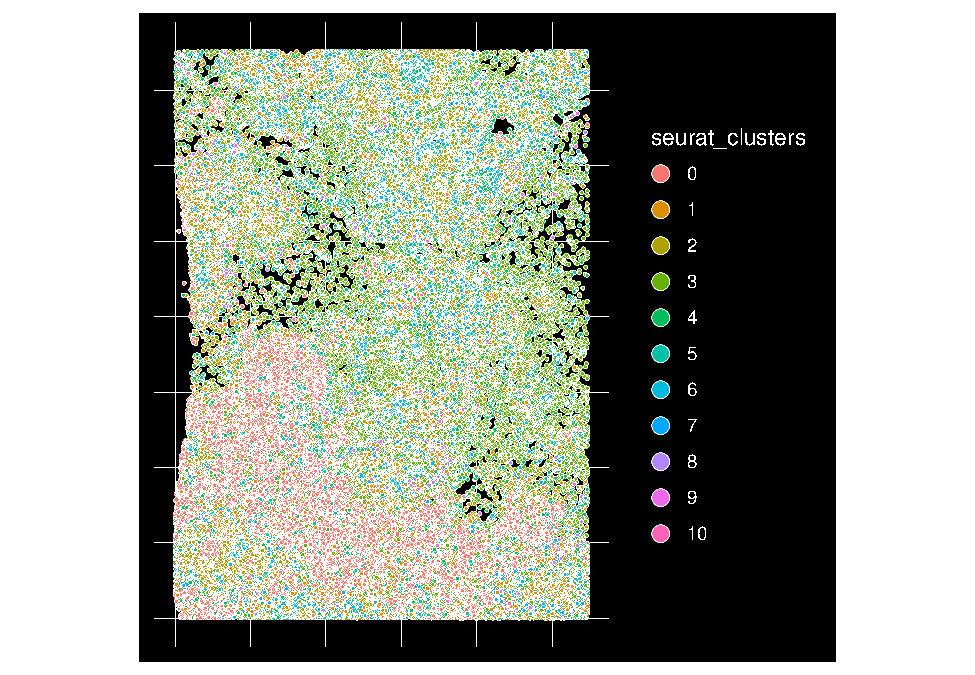
\includegraphics[keepaspectratio]{Sample_report_DFCI_files/figure-latex/unnamed-chunk-9-1.pdf}}

\begin{Shaded}
\begin{Highlighting}[]
\FunctionTok{ggsave}\NormalTok{(}\StringTok{"Spatial\_Clusters.png"}\NormalTok{, }\AttributeTok{width =} \DecValTok{6}\NormalTok{, }\AttributeTok{height =} \DecValTok{6}\NormalTok{)}

\CommentTok{\# Spatial plot of cell types}
\FunctionTok{ImageDimPlot}\NormalTok{(xenium.obj, }\AttributeTok{group.by =} \StringTok{"cell\_type"}\NormalTok{, }\AttributeTok{size =} \FloatTok{0.9}\NormalTok{)}
\end{Highlighting}
\end{Shaded}

\pandocbounded{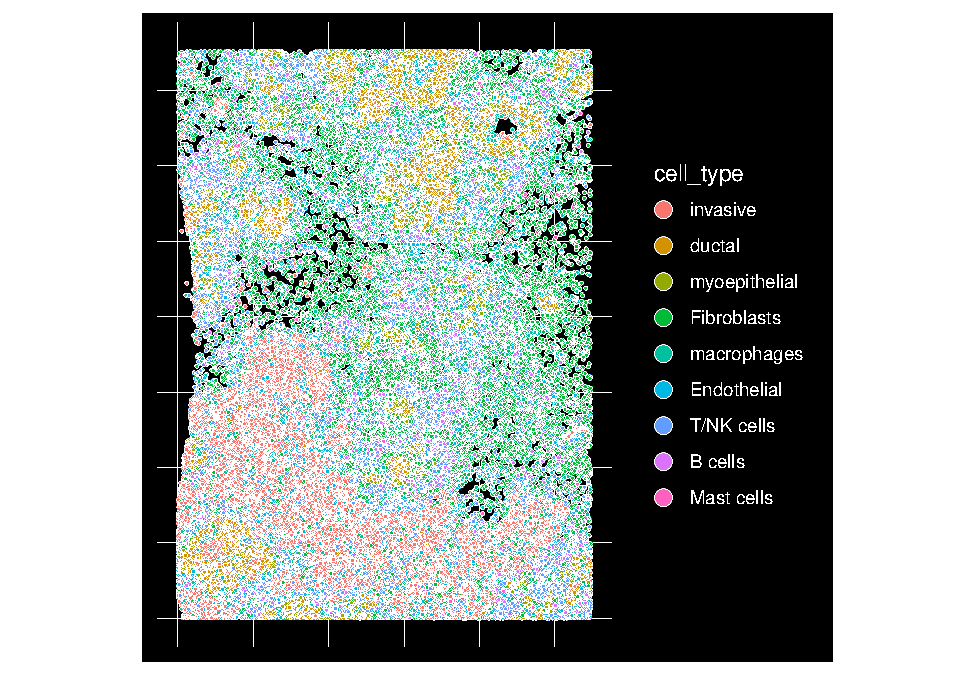
\includegraphics[keepaspectratio]{Sample_report_DFCI_files/figure-latex/unnamed-chunk-9-2.pdf}}

\begin{Shaded}
\begin{Highlighting}[]
\FunctionTok{ggsave}\NormalTok{(}\StringTok{"Spatial\_CellTypes.png"}\NormalTok{, }\AttributeTok{width =} \DecValTok{6}\NormalTok{, }\AttributeTok{height =} \DecValTok{6}\NormalTok{)}

\CommentTok{\# Gene expression spatial plots}
\FunctionTok{ImageFeaturePlot}\NormalTok{(xenium.obj, }\AttributeTok{features =} \StringTok{"FASN"}\NormalTok{, }\AttributeTok{cols =} \FunctionTok{c}\NormalTok{(}\StringTok{"white"}\NormalTok{, }\StringTok{"red"}\NormalTok{))}
\end{Highlighting}
\end{Shaded}

\pandocbounded{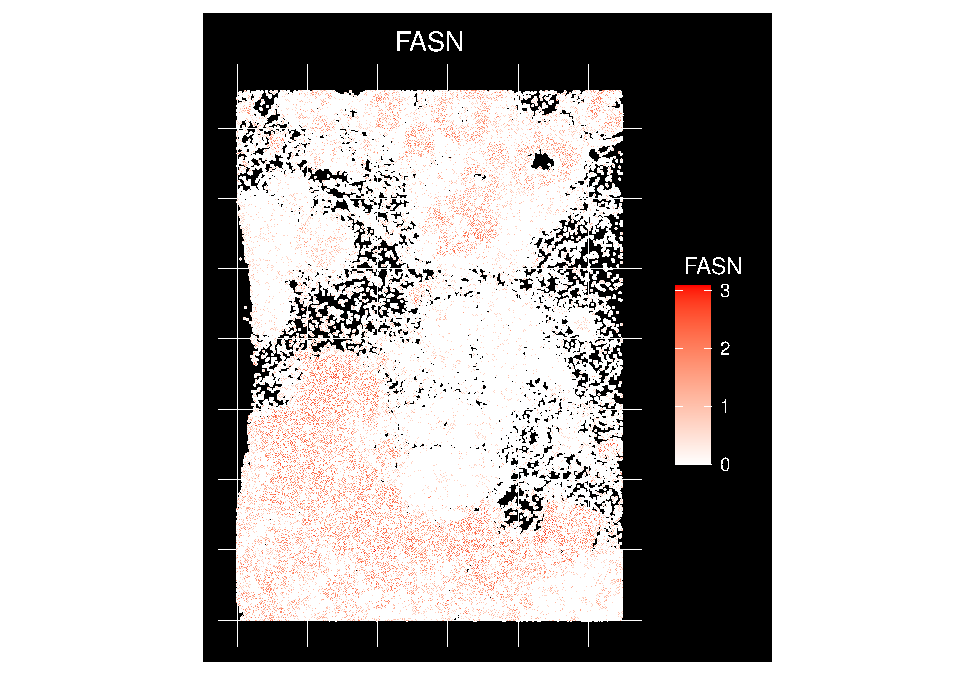
\includegraphics[keepaspectratio]{Sample_report_DFCI_files/figure-latex/unnamed-chunk-9-3.pdf}}

\begin{Shaded}
\begin{Highlighting}[]
\FunctionTok{ggsave}\NormalTok{(}\StringTok{"Spatial\_FASN.png"}\NormalTok{, }\AttributeTok{width =} \DecValTok{6}\NormalTok{, }\AttributeTok{height =} \DecValTok{6}\NormalTok{)}

\FunctionTok{ImageFeaturePlot}\NormalTok{(xenium.obj, }\AttributeTok{features =} \StringTok{"CEACAM6"}\NormalTok{, }\AttributeTok{cols =} \FunctionTok{c}\NormalTok{(}\StringTok{"blue"}\NormalTok{, }\StringTok{"red"}\NormalTok{))}
\end{Highlighting}
\end{Shaded}

\pandocbounded{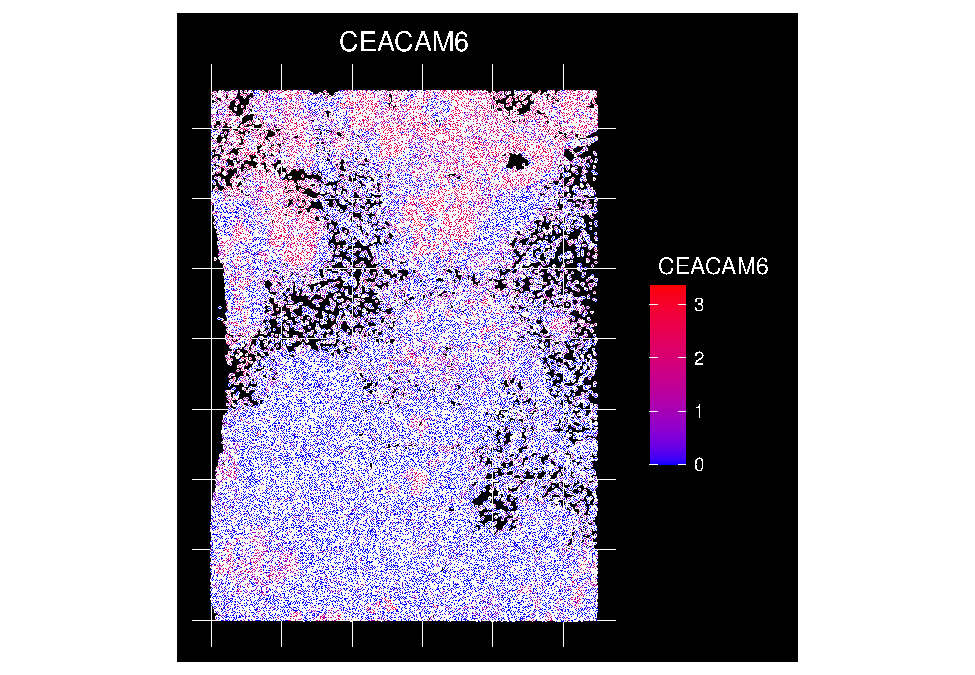
\includegraphics[keepaspectratio]{Sample_report_DFCI_files/figure-latex/unnamed-chunk-9-4.pdf}}

\begin{Shaded}
\begin{Highlighting}[]
\FunctionTok{ggsave}\NormalTok{(}\StringTok{"Spatial\_CEACAM6.png"}\NormalTok{, }\AttributeTok{width =} \DecValTok{6}\NormalTok{, }\AttributeTok{height =} \DecValTok{6}\NormalTok{)}

\CommentTok{\# Tumor{-}specific marker genes on spatial coordinates}
\FunctionTok{ImageDimPlot}\NormalTok{(xenium.obj, }\AttributeTok{fov =} \StringTok{"fov"}\NormalTok{, }\AttributeTok{nmols =} \DecValTok{20000}\NormalTok{, }\AttributeTok{axes =} \ConstantTok{TRUE}\NormalTok{,}
             \AttributeTok{molecules =} \FunctionTok{c}\NormalTok{(}\StringTok{"CEACAM6"}\NormalTok{, }\StringTok{"FASN"}\NormalTok{))}
\end{Highlighting}
\end{Shaded}

\pandocbounded{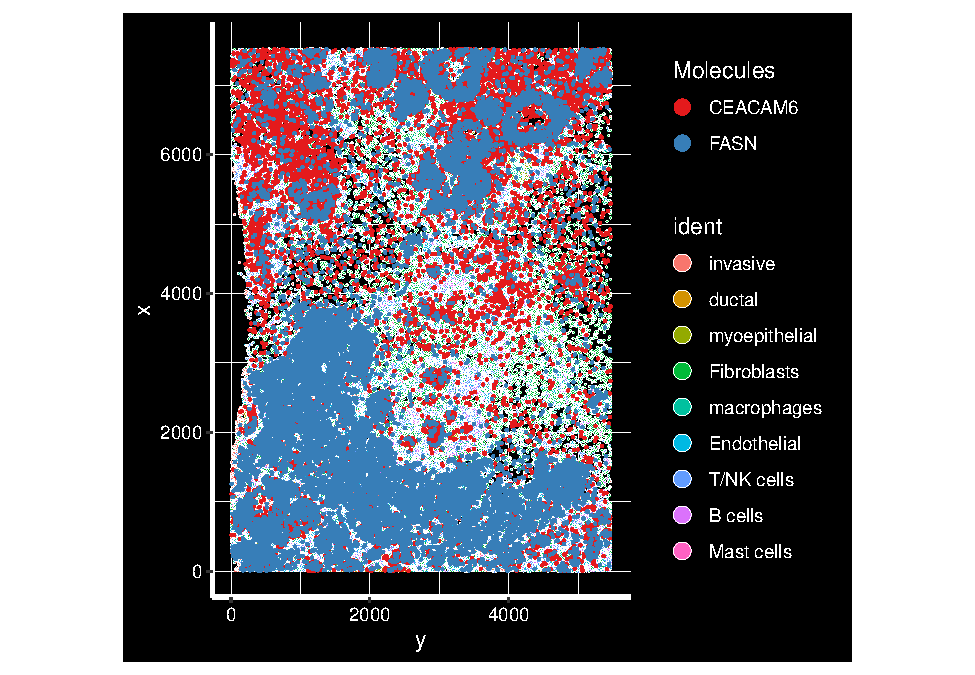
\includegraphics[keepaspectratio]{Sample_report_DFCI_files/figure-latex/unnamed-chunk-9-5.pdf}}

\begin{Shaded}
\begin{Highlighting}[]
\FunctionTok{ggsave}\NormalTok{(}\StringTok{"Spatial\_TumorMarkers.png"}\NormalTok{, }\AttributeTok{width =} \DecValTok{6}\NormalTok{, }\AttributeTok{height =} \DecValTok{6}\NormalTok{)}
\end{Highlighting}
\end{Shaded}

\subsection{Results}\label{results}

\section{Results}\label{results-1}

The analysis of the Xenium Human Breast Cancer Dataset provided key
insights into cellular composition and spatial organization:

\begin{enumerate}
\def\labelenumi{\arabic{enumi}.}
\tightlist
\item
  \textbf{Cell Type Identification}

  \begin{itemize}
  \tightlist
  \item
    Clustering identified distinct populations, annotated as invasive
    and ductal carcinoma cells, myoepithelial cells, fibroblasts,
    macrophages, endothelial cells, T/NK cells, B cells, and mast cells.
  \item
    Marker gene expression validated these annotations (e.g., FASN for
    invasive tumors {[}1{]}, CEACAM6 for ductal carcinoma {[}2{]}). See
    the table below for key markers:
  \end{itemize}

  \begin{longtable}[]{@{}lll@{}}
  \toprule\noalign{}
  Cell Type & Marker Genes & Reference \\
  \midrule\noalign{}
  \endhead
  \bottomrule\noalign{}
  \endlastfoot
  Invasive Tumor & FASN & Swinnen et al., 2006 {[}1{]} \\
  Ductal Carcinoma & CEACAM6 & Blumenthal et al., 2007 {[}2{]} \\
  B Cells & MS4A1, CD79A & Standard markers \\
  Macrophages & ITGAX & Standard markers \\
  T/NK Cells & CD3E, CD4, CD8A, NKG7 & Standard markers \\
  Endothelial & PECAM1 & Standard markers \\
  Myoepithelial & KRT15 & Standard markers \\
  Fibroblasts & LUM & Standard markers \\
  Mast Cells & KIT & Standard markers \\
  \end{longtable}
\item
  \textbf{Spatial Organization}

  \begin{itemize}
  \tightlist
  \item
    The spatial plot (\texttt{Spatial\_TumorMarkers.png}) revealed
    invasive carcinoma cells concentrated in peripheral regions,
    potentially marking tumor boundaries, while ductal carcinoma cells
    aligned with central ductal structures (see Figure 1).
  \item
    Immune cells (macrophages, T/NK cells) were dispersed throughout the
    tissue, suggesting infiltration into the tumor microenvironment,
    consistent with immune surveillance roles {[}3{]}.
  \end{itemize}

  \begin{figure}
  \centering
  \pandocbounded{\includegraphics[keepaspectratio]{Spatial_TumorMarkers.png}}
  \caption{Figure 1: Spatial distribution of tumor markers CEACAM6
  (ductal) and FASN (invasive)}
  \end{figure}
\item
  \textbf{Gene Expression Patterns}

  \begin{itemize}
  \tightlist
  \item
    FASN expression was elevated in invasive regions
    (\texttt{Spatial\_FASN.png}), aligning with its role in lipid
    metabolism supporting tumor growth {[}1{]}.
  \item
    CEACAM6 marked ductal carcinoma areas
    (\texttt{Spatial\_CEACAM6.png}), consistent with its association
    with epithelial-derived cancers {[}2{]}.
  \end{itemize}
\end{enumerate}

These findings underscore the cellular diversity and spatial
architecture of the breast cancer microenvironment, with implications
for tumor progression and immune interactions.

\begin{center}\rule{0.5\linewidth}{0.5pt}\end{center}

\subsection{Conclusion}\label{conclusion}

This spatial transcriptomics analysis demonstrates the utility of the
Xenium platform in dissecting the breast cancer tumor microenvironment.
By combining gene expression with spatial data, I identified key cell
types and their distributions, offering insights into tumor-immune
interactions and potential therapeutic targets.The elevated FAS
expression in invasive regions underscores its metabolic role,
suggesting avenues for targeting lipid metabolism in cancer therapy.
Future work could integrate additional datasets or functional assays to
validate these findings and explore clinical implications.

\begin{center}\rule{0.5\linewidth}{0.5pt}\end{center}

\subsection{References}\label{references}

\begin{enumerate}
\def\labelenumi{\arabic{enumi}.}
\tightlist
\item
  Swinnen, J. V., et al.~(2006). ``Fatty acid synthase drives the growth
  of prostate cancer cells.'' \emph{Cancer Research}, 66(8), 3814-3820.
\item
  Blumenthal, R. D., et al.~(2007). ``Carcinoembryonic antigen (CEA) and
  CEACAM6 in cancer progression.'' \emph{Cancer Biology \& Therapy},
  6(6), 831-837.
\item
  Hanahan, D., \& Weinberg, R. A. (2011). ``Hallmarks of cancer: The
  next generation.'' \emph{Cell}, 144(5), 646-674.
\end{enumerate}

\begin{center}\rule{0.5\linewidth}{0.5pt}\end{center}

\end{document}
